
\documentclass[a4paper,12pt]{article} % добавить leqno в [] для нумерации слева

\usepackage[left=2cm,right=2cm,
top=2cm,bottom=2cm,bindingoffset=0cm]{geometry}

\usepackage[english, russian]{babel} % выбор языка для документа
\usepackage[utf8]{inputenc} % задание utf8 кодировки исходного tex файла
\usepackage[X2,T2A]{fontenc}        % кодировка


\usepackage{amsmath,amsfonts,amssymb,amsthm,mathtools} % AMS
\usepackage{icomma} 
\mathtoolsset{showonlyrefs=true} % Показывать номера только у тех формул, на которые есть \eqref{} в тексте.
\usepackage{euscript}	 % Шрифт Евклид
\usepackage{mathrsfs} % Красивый матшрифт
\usepackage{enumitem}
\usepackage{siunitx}
\usepackage{tikz} % To generate the plot from csv
\usepackage{pgfplots}

\usepackage{graphicx}
\usepackage{subcaption}

%%% Заголовок
\author{}
\title{Корпоративные финансы}
\date{}

\newcommand{\latinword}[1]{\textsf{\itshape #1}}%

\begin{document}

\maketitle

\section{Введение: рынки капитала, потребление, инвестиции}
	
\subsection{Потребление и инвестиции без рынка капитала}

MRS - Marginal Rate of Substitution - между потреблением сегодня и завтра

MRT - Marginal Rate of Transformation -  The slope of a line tangent to curve
ABX is the rate at which a dollar of consumption foregone today is transformed
by productive investment into a dollar of consumption tomorrow.  An individual endowed with a resource
bundle $ (y_0, y_1) $ that has utility $ U_1 $ can move along the production opportunity set
to point $ B $, where the indifference curve is tangent to it and he or she receives the
maximum attainable utility, $ U_2 $. Because current consumption, $ C_0 $, is less than the
beginning-of-period endowment, $ y_0 $, the individual has chosen to invest. The amount
of investment is $ y_0 — C_0 $. 

\begin{figure}[h!]
	\centering
	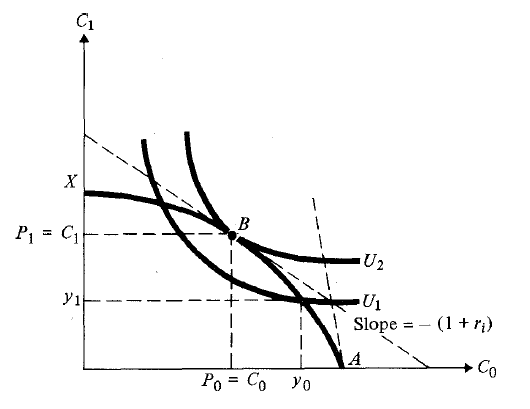
\includegraphics[width=0.5\linewidth]{screenshot001}
	\caption{Задача о распределении потребления во времени}
	\label{fig:screenshot001}
\end{figure}

КПВ - Кривая производственных возможностей - характеризуется убывающим предельным продуктом MP

$ MRS = MRT $ - необходимое и достаточное условие внутреннего о оптимума 

$ \rho $ - норма межвременных предпочтений

$ i $
- доходность производственных инвестиций

The individual decision maker starts with an
initial endowment $ (y_0, y_1) $ and compares the marginal rate of return on a dollar of
productive investment (or disinvestment) with his or her subjective time preference.
If the rate on investment is greater (as it is in Fig. 1.5), he or she will gain utility by
making the investment. This process continues until the rate of return on the last
dollar of productive investment just equals the rate of subjective time preference (at
point B). Note that at point B the individual's consumption in each time period is
exactly equal to the output from production.

Два типа агентов: "терпеливые" и "нетерпеливые". У всех первоначальные запасы одинаковые, но из-за различных межвременных предпочтений разные оптимальные точки

 \begin{figure}[h!]
 	\centering
 	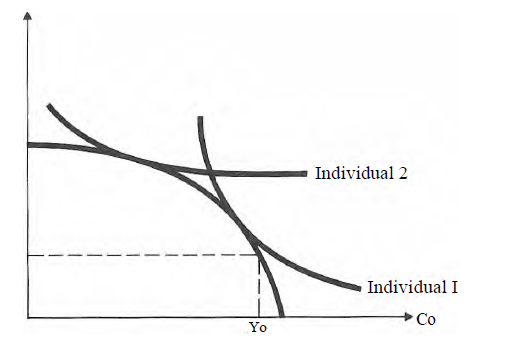
\includegraphics[width=0.5\linewidth]{screenshot002}
 	\caption{Individuals with different indifference curves choose  		different production/consumption patterns.}
 	\label{fig:screenshot002}
 \end{figure}
 
\subsection{Потребление и инвестиции с рынком капитала} 

Проблема (Фишер): 
Есть некторые пропорции, влияющие на выбор оптимума помимо межвременных предпочтений. Проблема неэффективности решается обменом по рыночным ценам. 

Введем рынок капитала. Межвременной обмен потребительских наборов может быть реализован через возможность неограниченно ссужать и занимать по единой рыночной ставке процента $ r $.

\subsubsection{Случай без КПВ}

Пусть $ r > 0 $, производство отсутствует $ \Rightarrow $ есть запас, но КПВ отсутствует 

Есть возможность занимать  $ \Rightarrow  $ линия рынка капитала (Capital Market Line) 

\begin{figure}[h!]
	\centering
	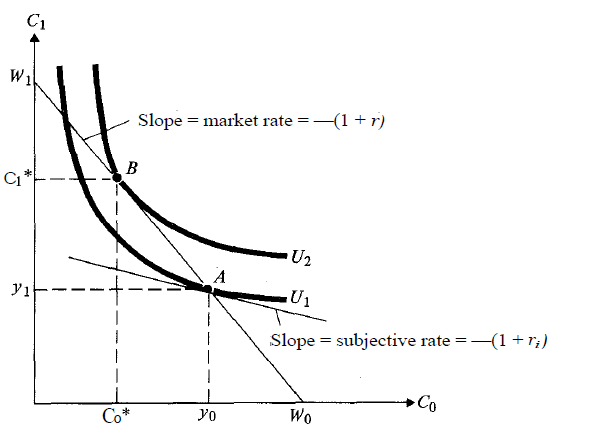
\includegraphics[width=0.5\linewidth]{screenshot003}
	\caption{CML}
	\label{fig:screenshot003}
\end{figure}

With an initial endowment of $ (y_0, y_1) $ that has utility
equal to $ U_1 $, we can reach any point along the market line by borrowing or lending
at the market interest rate plus repaying the principal amount. 



$ w_0 = y_0 +  \dfrac{y_1}{1+r} $

$ w_1 = y_0(1+r) + y_1$

$ w_0w_1 $ - CML

Финансовые рынки повышают благосостояние в терминах полезности 

\subsubsection{Случай с КПВ}

Введем производство, затем обмен на рынке

\begin{figure}[h!]
	\centering
	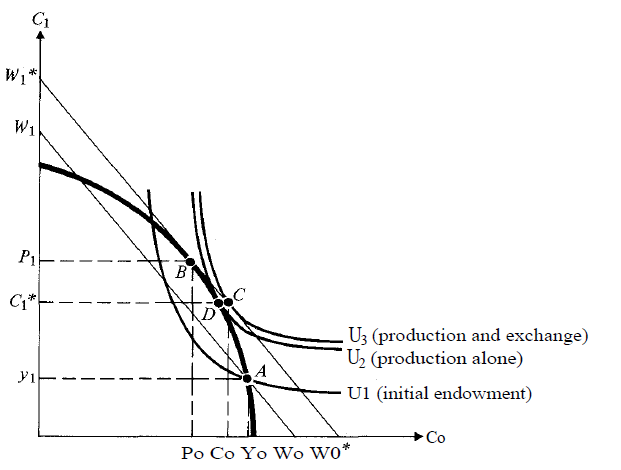
\includegraphics[width=0.5\linewidth]{screenshot004}
	\caption{Production and consumption with capital markets}
	\label{fig:screenshot004}
\end{figure}

$ A $
- точка первоначального наделения (не опт., т.к. можно улучшить передвижением вдоль КПВ и CML). Оба варианта дают доходность выше, чем $ \rho $ 

Выбираем производство, приносящее большую доходность

В точке $ A: i > r > \rho $ 

$ D $ -  точка касания КПВ и кривой безразличия

В точке $ D: i = \rho \Leftrightarrow MRT = MRS $, причем в отстутствие рынка капитала, мы бы остановились в этой точке. Но в точке $D: i > r \Rightarrow $ касательная более крутая, чем CML. Ставка на рынке меньше, чем доходность (занимать на рынке дешево) $ \Rightarrow  $  наращиваем производство до точки $ B $, где $r = i $

$ B $
 - точка касания КПВ и линии, параллельной CML (оптимум производства)
 
В точке  $ B $ выпуск $ (P_0,P_1) $,  а богатство $w_0^* > w_0  $. Но в точке $ B: \rho > r $

$ C $ - оптимум потребления. При $ \rho > i $ будем потреблять больше чем произведено $ C_0 > P_0 $. 
Беря взаймы, сможем достигнуть точки $ С $, поскольку при новой CML мы можем достигнуть любую точку на ней. 

$ r = \rho $ -  Market rate of return  = Time preference 




\paragraph{Современный рынок капитала:}

\begin{enumerate}
	\item Большое число продавцов и покупателей финансовых активов (price-taker)
	\item Информационная прозрачность, отсутствие асимметрии информации
	\item Отсутствие налогов и других издержек, искажающих трений (брокерская комиссия)
\end{enumerate}  
  
  \paragraph{Полный рынок капитала - }
  рынок, на котором существует определённая легко получаемые ценное бумага на каждый возможный случай 
  
 
\paragraph{Теорема Фишера (о разделении инвестирования и потребления):}

В ситуации современных и полных рынков капитала решение о производстве определяется исключительно объективными рыночными условиями и не зависит от субъективных предпочтений   индивидов, которые влияют на из решение о потреблении

Процесс принятия решений о производстве и рыночном обмене (два отдельных решения):

\begin{enumerate}
	\item Оптимальное решение о производстве: $ i = r $, предельная доходность инвестиций  = рыночному проценту (не зависит от предпочтений)
	\item Решение об оптимальном потреблении с помощью рынка капитала: $ \rho = r $ 
\end{enumerate}


 Важное применение:   принятие инвестиционных решений может быть делегировано менеджерам
 
 In equilibrium, the marginal rate of substitution for all investors is equal to the
 market rate of interest, and this in turn is equal to the marginal rate of transformation
 for productive investment. Thus all individuals use the same time value of money (i.e., the same market-determined
 objective interest rate) in making their production/investment decisions.
 
 В равновесии  все используют одинаковые time value of money: $ MRS_i = MRS_j = -(1+r) = MRT $ 

  Рынки капитала позволяют эффективно перераспределять средства от заемщиков к занимателям. 
    
 \subsection{ Нарушение разделения Фишера и транзакционные издержки}
  
  \subsubsection{Проблема делегирования}
  
    Market friction из-за асимметрии 
  
  В реальной жизни ставка $ r $ не одна -   теперь индивиды выбирают разные уровни производства 
    
  \begin{figure}[h!]
  	\centering
  	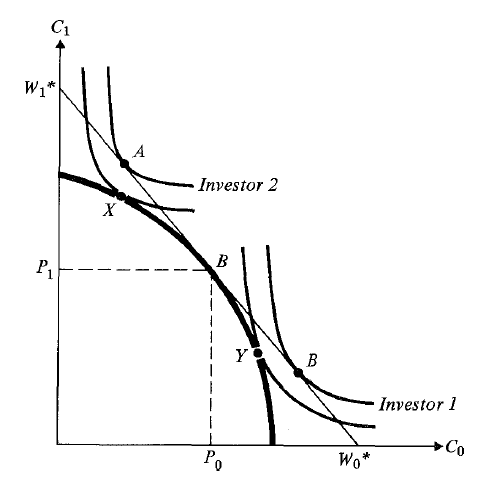
\includegraphics[width=0.4\linewidth]{screenshot005}
  	\caption{The investment decision is independent of individual preferences.}
  	\label{fig:screenshot005}
  \end{figure}
  
 $  X, Y $ - производственные решения
 
 $ A, B $ - потребление
  
    Разные CML: $ r_2> r_1 \Rightarrow $ разные оптимумы  $ \Rightarrow $    
    нельзя делегировать управление компанией стороннему  менеджеру 
    
    
    \newpage
    
    
 \section{Принятие инвестиционных решений в условиях определённости (Capital budgeting)}
 
    \paragraph{Предположение:}
  
  Ставка процента детерминированна (известна с определённостью $ \Rightarrow $ нет рисков)
  
  
  
  \paragraph{Цель: } 
  
  Максимизация приведённой стоимости потребления (богатства) на определённом временном горизонте 
    
  
Выбор индивидов принадлежит линии рынка капитала CML,  а значит менеджеру не нужно думать о различных предпочтениях акционеров
  
  
  \subsection{ Максимизация богатства акционеров}
  
\subsubsection{Дивиденды VS Прирост капитальный стоимости}

\[ S_0 = \sum_{i=1}^{\infty} \dfrac{Div_t}{(1+k_s)^t} \]
  
  где
 $ S_0 $  - богатство в нулевой период, 
  $ k_s $ -  требуемая нормы доходности на акции,  определяемая рынком
  
  Из формулы Гордона:
   
   \[ S_0 = \dfrac{Div_1}{(k_s-g)} =  \dfrac{Div_0 (1+g)}{(k_s-g)} \]
   
   где 
  $ g $  - темп  прироста дивидендов
  
  
  \paragraph{ Пример: }
  
  Пусть  $ Div_1 = 1 \$, k_s = 10 \%, g = 5 \%  $, тогда
  
   \[ S_0 = \dfrac{Div_1}{(k_s-g)} =  \dfrac{1 }{0.1-0.05} = 20 \]
  
  Через 5 лет акция будет стоить:
  
  \[ S_5 = \dfrac{Div_6}{(k_s-g)}  = \dfrac{Div_1(1+g)^5}{(k_s-g)}  \approx 25.5 \]
  
  The value of the stock at the end of the fifth year is the discounted value of all dividends
  from that time on.
  
  \[ S_0 =  \dfrac{Div_1}{(1 + k_s)} +  \dfrac{Div_1(1+g)}{(1+ k_s)^2} + ... +  \dfrac{Div_1(1+g)^4}{(1+ k_s)^5}  + \dfrac{S_5}{(1+ k_s)^5}  \approx 20.01 \]
  
  
  
  В отсутствие налоговых искажений и при  детерминированности ставок нет разницы между выплатой дивидентов и приростом капитальный стоимости.
  
  
  \subsubsection{Прибыль}
  
   \paragraph{Экономическая прибыль:  }
   
   \[ Div_t = TR_t - TC_t - I_t \]
   
    Cумма, которая может быть направлена на выплаты дивидендов
   
\paragraph{   Бухгалтерская прибыль: }
   
   \[ NI_t = TR_t - TC_t - dep_t \]

где $ NI $ - net income, $ dep $ -   
    амортизация 
    
    \[ Div_t = \Delta A_t\]
    
  где     $ A_t $ - 
    изменения стоимости актива 
    
    
   Бухгалтерский подход в отличие от экономического не учитывает момент возникновения денежного потока, а также расходов на инвестиции, что  важно, так как существует дисконтирование 
   
   
   \subsection{Метод планирования капитальных вложений} 
   
   Работаем с "идеальным" миром 
   
   Принципы принятия решений:
   
   \begin{enumerate}
   	\item  Нужно учитывать все денежные потоки по проекту 
   	\item  Нужно дисконтировать потоки денежных средств по альтернативной  стоимости
   	\item  Выбор из взаимоисключающих проектов, если нужно выбрать только один 
   	\item Принцип аддитивности стоимости: $ V = \sum_{i=1}^{N} V_j  $ рассмотрение проектов отдельно друг от друга (нет сложных комбинаций проектов) 
   	
   \end{enumerate}
   
    
    \subsubsection{Методы определения срока окупаемости долгосрочных инвестиций (Payback Method)} 
       
   \paragraph{ Критерий выбора:     }
  выбираем проект, который быстрее позволит "вернуть" первоначальные инвестиции
  
\paragraph{    Недостатки:  }
   
   \begin{itemize}
   	\item  Учитываем не все потоки по проекту 
   	\item   Отсутствие дисконтирования денежных потоков
   \end{itemize}
   
 \subsubsection{Бухгалтерская норма доходности (Accounting Rate of Return)} 

\[ ARR  = \dfrac{Average \ after-tax \ profit}{Initial \ outlay}  \]

   \paragraph{ Критерий выбора:     }  наибольший ARR
   
    \paragraph{    Недостатки:  }
    
    \begin{itemize}
    	\item  Использование бухгалтерской прибыли,  а не  денежных потоков 
 \item   	Не учитывается временная ценность денег (хронология выплат  неважна -  нет дисконтирования)  
    \end{itemize}
    
    \subsubsection{Метод чистой приведённой стоимости (Net Present Value) }
    
    Чистая приведенная стоимость (NPV) – сумма первоначальных вложений и приведенной стоимости всех будущих денежных потоков проекта
        (сколько заработано в сегодняшних деньгах):
    
    \[ NPV = \sum_{i=1}^{N} \dfrac{Cash \ flow_t}{(1+ Discount \ factor)^t} -I_0 \]
    где $ CF_0 = I_0 $
    

 
\paragraph{ Правила принятия решений по NPV:}
 \begin{enumerate}
 	\item Если проекты независимые, то принимается любой проект $ NPV \geq 0 $
 	\item Если проекты альтернативные, то выбирается с max $  NPV $.
 	 \item Если существует инвестиционная политика компании, то принимаются все проекты с $ NPV > $ целевого значения.
 \end{enumerate}
 
\paragraph{ Достоинства:}
\begin{enumerate}
	\item Учитывает стоимость денег во времени
		\item Легко рассчитать на компьютере
	 	\item Содержит некий учет ликвидности
\end{enumerate}
  
 \paragraph{    Недостатки:  }
 \begin{enumerate}
 	\item Проблемы с выбором ставки дисконтирования: можно выбрать по ставке, сложившейся на фин.рынке или по ставке альтернативных вложений (банк)
 	\item Пассивное управление проектом
 	\item Нет учета вне проектных возможностей (не учитывает положительные экстерналии)
 	
 \end{enumerate}
 
  
  \subsubsection{Внутренняя норма доходности (Internal Rate of Return) }
  
$   IRR $  - такая ставка процента при которой $ NPV = 0  $
  
  \[  \sum_{i=1}^{N} \dfrac{CF_t}{(1+ IRR)^t} -I_0 = 0 \] 
  
   \paragraph{ Критерий выбора:     }  IRR должен быть выше, чем
  альтернативная стоимость средств
  
  \begin{figure}[h!]
  	\centering
  	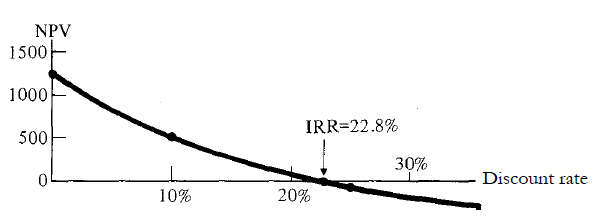
\includegraphics[width=0.7\linewidth]{screenshot006}
  	\caption{NPV of project C at different discount rates}
  	\label{fig:screenshot006}
  \end{figure}
  
   \paragraph{ Недостатки:     }

\begin{enumerate}
	\item 
 Нет дисконтирования  по альтернативной стоимости средств 
 	\item 
 Реинвестирование CF по ставке IRR  не является реалистичным, так как IRR не имеет ничего общего с рыночной ставкой  процента 
 	\item 
 Не выполняется принцип аддитивной стоимости (нельзя складывать между собой CF дисконтированные по-разным IRR) 
  	\item Multiple rates of
  	return if the stream of estimated cash flows changes sign more than once

\end{enumerate}

   \paragraph{ Из экономических соображений NPV рассчитывается иначе:     }
   
   Для второго периода: 
   
   \[ [-1600I_0(1+IRR) + 10000](1 + k) - 10000  = 0  \]

при $ k = 0.1 $ - рыночная ставка, по которой мы можем реинвестировать полученные в первом периоде деньги

\[ IRR = - 43 \%  \Rightarrow\]  в проект можно вложиться только на 2 года

При $ NPV  = 0 $ можно вкладываться каждый год




\subsection{Денежные потоки при планировании капитальных вложений}

\paragraph{ Revenue}
 
 - (Variable Cost + Fixed Cash Cost) 
 
 - dep - амортизация
 
$  \Downarrow $
 
\paragraph{ Earnings Before Interest and Tax } (Прибыль до выплаты процента по долгам и до налогообложения) 
 
 -  Interest expenses $ k_d D $,  где $ k_d   $ - норма доходности
 
 - Taxes 
 
 $  \Downarrow $
 
 \paragraph{Net Income }
 (Выплаты дивидендов/ реинвестирование/ перераспределенная прибыль       $ \Rightarrow $ собственный капитал $ \uparrow $)

\paragraph{
Свободный денежный поток фирмы (Free CF to firm) 
}

 \[ FCF = \Delta Rev - \Delta Costs - \Delta I - \tau_c (\Delta Rev - \Delta Costs - \Delta Dep )  = EBIT(1-\tau_c) + \Delta Dep - \Delta I \]
 
 где $ \tau_c $ - 
предельная ставка налога, $ I $
- инвестиции 


\paragraph{Средневзвешенная стоимость капитала (Weighted Average Cost of Capital)} 

\[ WACC = k_b \dfrac{B}{B+E} (1-\tau_c) +  k_e \dfrac{E}{B+E} \]

где $  k_b $  - стоимость заемного капитала,
$ \dfrac{B}{B+E} $  - доля заемного капитала,  
$ B $ - заемный капитал (bonds), $ E $ - собственный капитал (equity),   $  k_e $  - требуемая доходность  собственного капитала 

По WACC дисконтируются денежные потоки фирмы 

\section{Принятие инвестиционных решений в случае неопределенности}

В реальности надо делать выбор между активами с неизвестными фактическими доходностями.  
Обычно работаем с "хорошими" предпочтениями - с рискофобами

\subsection{Случай одного актива }

Rate of Return  

\[ R = \dfrac{W - I}{ I} \]

где $ R $ - доходность, $ I $ - инвестиции на начало периода, $ W $ - валовый доход на конец периода 

$ W = (1+R) I  $ - формулировка в терминах будущей стоимости 

$ I = (1+R)^{-1} W $ - формулировка в терминах в текущей стоимости 

Если речь идёт о безрисковом инструменте,  то мы знаем R.  
Если W неизвестна, то
 фактически мы будем работать со случайными величинами.
 
  Акция - инструмент, случайная величина - цена акции на конец периода 
  
  \subsubsection{Математическая статистка}

\paragraph{Математическое ожидание:}

\[ E(\tilde{X})  = \sum_{i=1}^{N} p_i X_i  \]

Если $ \tilde{P} $ - цена актива, $ I = P_0 $ - цена в начале периода, то 

\[ E (\tilde{R}) = \dfrac{\tilde{P} - P_0}{P_0} \]

\paragraph{Дисперсия}

\[ Var(\tilde{X}) = \sigma^2 = E [(X_i - E(\tilde{X}))^2] = \sum_{i=1}^{N} p_i (X_i - E(\tilde{X}))^2 \] 

\paragraph{Дисперсия доходности:}  \[ Var(\tilde{R}) = \dfrac{\sigma^2(\tilde{P})}{P_{0}^{2}}\]


\paragraph{Корреляция доходности}

\[ 0 \leq r_{XY} = \dfrac{cov(X,Y)}{\sigma_X\sigma_Y} \leq 1 \]

  Пусть в $ X $  мы вкладываем $  a \% $ нашего богатства, а в $ Y - b=(1-a) \% $.
  
  \[ \sigma^2(R_p) = \sigma^2(aX+bY)  = a^2\sigma^2(X) + b^2\sigma^2(Y) + 2 ab r_{XY} \sigma(X)  \sigma(Y)    \]

\subsection{Измерение риска и доходности портфеля}

 Часто для простоты предполагает, что доходность распределена нормально 
 
 \[ R \sim N(\sigma^2) \Rightarrow f(R) =  \dfrac{1}{\sigma \sqrt{2\pi}} e^{-\dfrac{1}{2} \left[\left( \dfrac{R-\mu}{\sigma}\right) ^2\right]} \]
 
 Если Z - центрировано:
 
 \[ Z =  \dfrac{R-\mu}{\sigma} \Rightarrow f(Z) =  \dfrac{1}{ \sqrt{2\pi}} e^{-\frac{1}{2} Z^2} \]
 
 
\subsubsection{ Портфель с минимальной дисперсией }
  
\[   \sigma^2(R_p) = a^2\sigma^2_X + (1-a)^2\sigma^2_Y + 2 a(1-a) r_{XY} \sigma_X  \sigma_Y  \longrightarrow \max_{a \in [0;1] }
   \]
   Для внутреннего оптимума:
   
  \[ \dfrac{\partial  \sigma^2(R_p) }{\partial a}  = 0\]
  
  Откуда:
  \[  a^{*} = \dfrac{ \sigma^2_Y - r_{XY} \sigma_X  \sigma_Y  }{\sigma^2_X + \sigma^2_Y - r_{XY} \sigma_X  \sigma_Y }, a^{*} \in (0;1) \]
  
  
 
 
 
 
   \begin{figure}[h!]
   	\centering
   	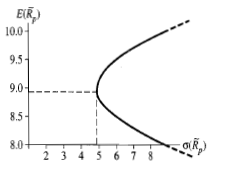
\includegraphics[width=0.4\linewidth]{screenshot007}
   	\caption{Trade-off between mean and standard deviation.}
   	\label{fig:screenshot007}
   \end{figure}
   
   
   
   \subsection{Портфельная теория (Маргарец, 1952)}
   
    
\paragraph{   Глобальная цель инвестора:}  Выбрать некоторый портфель активов с определёнными характеристиками по ожидаемой  доходности к риску

 
\paragraph{Диверсификация портфеля} - распределение инвестиций   с целью понижения общего уровня риска инвестиций.  Поскольку инвестор - рискофоб, почти наверное он будет диверсифицировать риски инвестиции 
 
 
   \begin{figure}[h!]
 	\centering
 	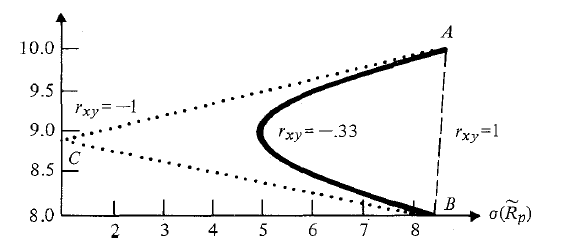
\includegraphics[width=0.7\linewidth]{screenshot008}
 	\caption{Risk-return trade-offs for two assets.}
 	\label{fig:screenshot008}
 \end{figure}
 
 \subsubsection{Perfectly Correlated Assets}
 
Если $ r_{XY}  = 1 $, то $   \sigma^2(R_p) = a^2\sigma^2_X + (1-a)^2\sigma^2_Y + 2 a(1-a) \sigma_X  \sigma_Y  = [a\sigma_X + (1-a)\sigma_Y]^2 $

  
  
  
    \[  a^{*} = \dfrac{ \sigma^2_Y -  \sigma_X  \sigma_Y  }{\sigma^2_X + \sigma^2_Y -  \sigma_X  \sigma_Y } =  \dfrac{ \sigma_Y  }{\sigma_X -    \sigma_Y }  \]
  
  
  В "простом" мире не можем выходить в короткие позиции, 
   в "сложном" мире ($ a \in (-\infty; \infty ) $) может быть два корня 
   
 
   
   
   Вложение в  абсолютно коррелированые активы не позволяет снижать риски, т.к. нет возможности диверсификации 
   
   Trade-off между ожидаемой  доходностью и  риском - постоянная величина (прямая линия)
   
   \[ 
   Slope =
   \dfrac{d E(R_p)}{d \sigma (R_p) } = \dfrac{\dfrac{d E(R_p)}{d a}}{\dfrac{d \sigma (R_p)}{da} } = \dfrac{E(X)-E(Y)}{\sigma_X - \sigma_Y } \]
   
    
   
   
   
   \subsubsection{Perfectly Incorrelated Assets}
   
   Если $ r_{XY}  = -1 $, то $   \sigma^2(R_p) = a^2\sigma^2_X + (1-a)^2\sigma^2_Y -  2 a(1-a) \sigma_X  \sigma_Y  = [a\sigma_X - (1-a)\sigma_Y]^2  \Rightarrow  \sigma(R_p)  = \pm [a\sigma_X - (1-a)\sigma_Y] $ 
      
  Два корня - две линии: с положительным и с отрицательным наклоном, которые  пересекаются в точке $ C $ на вертикальной оси,  соответствующей портфелю с минимальной  дисперсией
  
   \[  a^{*} = \dfrac{ \sigma^2_Y +  \sigma_X  \sigma_Y  }{\sigma^2_X + \sigma^2_Y +  \sigma_X  \sigma_Y } =  \dfrac{ \sigma_Y  }{\sigma_X +    \sigma_Y }  \]
   
   В этом случае $ E(R_p) = \mu^{*}, \sigma (R_p) =  0 $
  
  
   \subsection{Эффективная  граница} 
  
  Эффективная граница (Efficiency Opportunity Set) -  это набор различных выборов (the set of mean-variance choices) из множества инвестиционных возможностей, где для заданной дисперсий никакая другая инвестиционная возможность не позволит получить более высокую жидами доходность
   
   \subsubsection{Случай двух рисковых активов}
   
   Безрискового актива нет, нет обмена и, следовательно,  возможности
  брать деньги в долг или одалживать 
  
   \begin{figure}[h!]
   	\centering
   	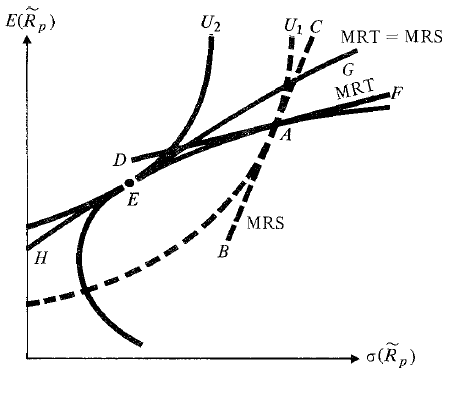
\includegraphics[width=0.5\linewidth]{screenshot009}
   	\caption{The utility maximizing choice equates the marginal rates of substitution and transformation.}
   	\label{fig:screenshot009}
   	
   	
   \end{figure}
   
   
   У разных агентов  разные точки выбора: 
   
   
\begin{figure}[h!]
	\centering
	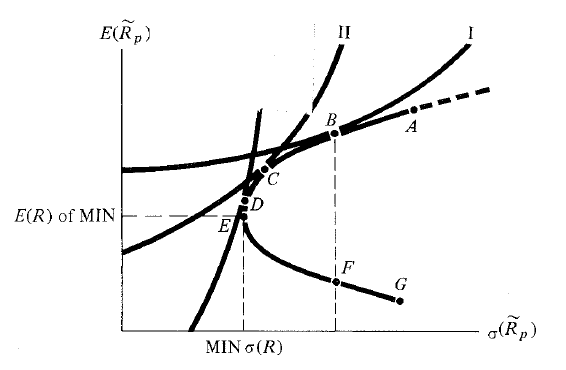
\includegraphics[width=0.5\linewidth]{screenshot010}
	\caption{Choices by investors with different indifference curves.}
	\label{fig:screenshot010}
\end{figure}
   
    \subsubsection{Случай одного рискового и одного безрискового актива
    }


   Пусть 
   $ R_f $  -  доходность безрискового актива, $ \sigma^2_{f}  = 0 \Leftrightarrow $ 
    можно давать деньги в долг
    
    \[ E(R_p) = aE(X) + bR_f \]
    
    \[ \sigma^2(R_p) = a^2 \sigma^2_{X} \Rightarrow  \sigma(R_p) = |a| \sigma_{X} \]
   
   
   \begin{figure}[h!]
   	\centering
   	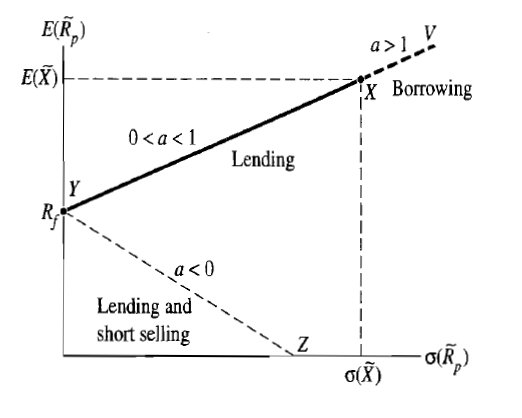
\includegraphics[width=0.5\linewidth]{screenshot011}
   	\caption{Opportunity set with one risky and one risk-free asset.}
   	\label{fig:screenshot011}
   \end{figure}
   
   При $ a > 1  $    
   занимаем деньги по $  R_f  $,  вкладываем всё в актив X 
   
   При $ 0 < a < 1  $    
   даем в долг и инвестируем в X 
   
    При $ a < 0  $ short-selling:     
   продаем X  и все деньги отдаем в долг 
   
   Для простоты: ставка по заимствованию, равна кредитной ставке и равна рисковой ставке 
   
    \[ 
    Slope =
    \dfrac{d E(R_p)}{d \sigma (R_p) } = \dfrac{\dfrac{d E(R_p)}{d a}}{\dfrac{d \sigma (R_p)}{da} } = \dfrac{E(X)-R_f}{\sigma_X } \]
    
     \subsubsection{Случай n рисковых активов
    }
    
    
    \[ E(R_p)  = \sum_{i=1}^{N} w_i E(R_i),    \sum_{i=1}^{N} w_i = 1 \]
    
    
        
        Множество инвестиционных возможностей  
        
           \begin{figure}[h!]
        	\centering
        	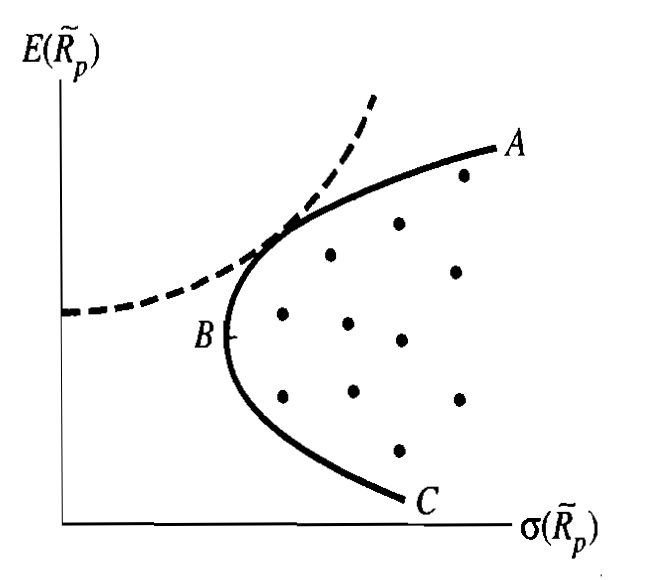
\includegraphics[width=0.4\linewidth]{screenshot012}
        	\caption{The investment opportunity set with
        		many risky assets}
        	\label{fig:screenshot012}
        \end{figure}
        
        
        
        
        В случае двух рисковых активов множество инвестиционных  возможностей - вогнутая  линия, а в случае $ n $  рисковых активов - та же линия плюс  всё, что внутри
   
   

   
   \subsubsection{Эффективное множество в случае n рисковых активов и одного безрискового актива    }
   
   
   \begin{figure}[h!]
   	\centering
   	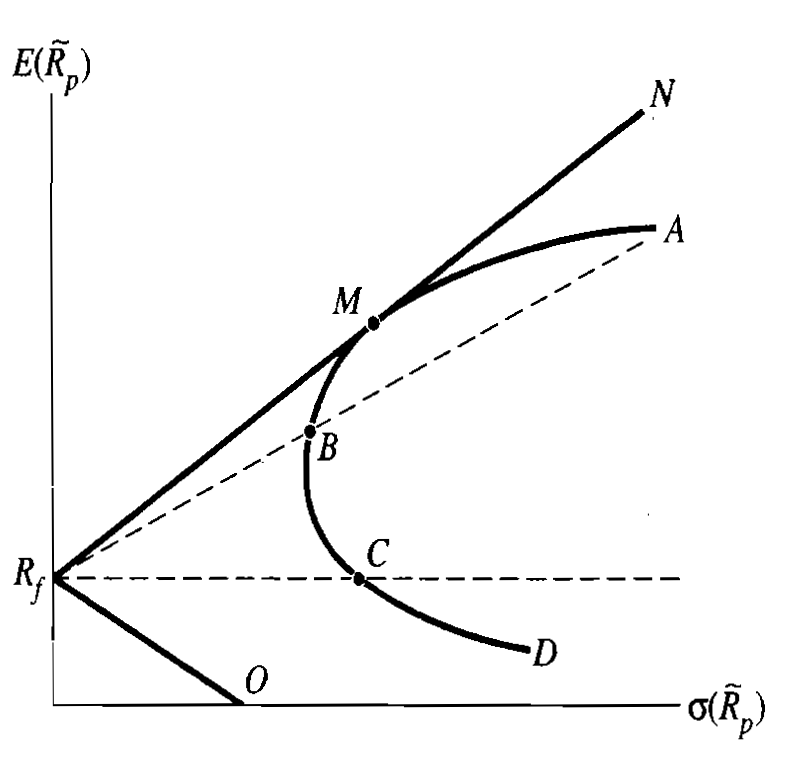
\includegraphics[width=0.4\linewidth]{screenshot013}
   	\caption{The efficient set with one risk-free and many risky assets.}
   	\label{fig:screenshot013}
   \end{figure}
   
   
    По аналогии с одним рисковым и одним безрисковым активом, проведем линию через $ R_f $  и любой из портфелей.
     Наилучшая  линия - та,  которая  касается границы инвестиционных возможностей. 
     Рыночный портфель $ M $ включает в себя все рисковые активы.
      
    
    \subsection{Capital Market Line}
      
      \begin{figure}[h!]
      	\centering
      	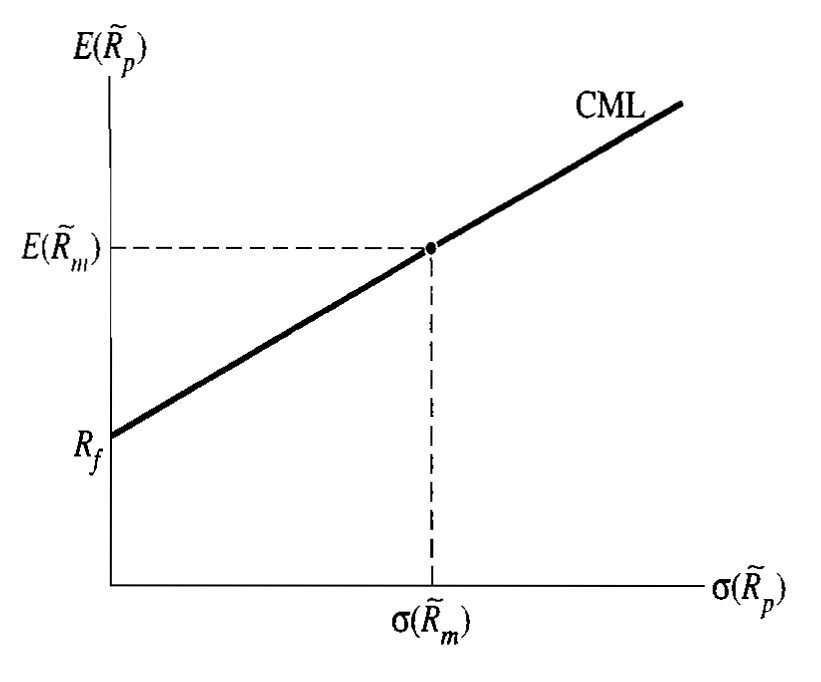
\includegraphics[width=0.4\linewidth]{screenshot014}
      	\caption{CML}
      	\label{fig:screenshot014}
      \end{figure}
      
      
      Если ожидания агентов однородны, то они будут сталкиваться с одним и тем же линейным эффективным множеством, называемым линией рынка капитала
      
      \[ E(R_p) = R_f + \underbrace{\dfrac{E(R_m)-R_f}{\sigma(R_m)}  \sigma (R_p) }_{\text{компенсация за риск}} \]
   
\section{Модель ценообразования финансовых активов (Capital Asset Pricing Model)} 

Цель: определить  цену риска по какому-либо активу (цена риска - премия за риск)

\subsubsection*{ Предпосылки:} 

 \begin{enumerate}
 	\item Инвесторы не склонны к риску максимизирует ожидаемую полезность своего богатства
 	\item  Инвесторы являются  price-takers и имеют одинаковые ожидания относительно доходности активов, которые совместно нормально распределены 
 	\item Существует безрисковая ставка процента и агенты могут неограниченно ссужать по ней или брать в займы
 	\item  Предложение каждого активно фиксировано (строго определёно), все активы торгуются  на рынке бесконечно делимы.  
 	\item Рынки активов лишены трений,  информация бесплатна и доступна одновременно всем инвесторам 
 	\item Рыночные несовершенства типа налогов, регулирования ограничений, коротких продаж отсутствуют 
 \end{enumerate}

Составим портфель,  который будет состоять из $ i $-ого рискового актива и рыночного портфеля $ M $ 

    \[ E(\tilde{R}_p) = aE(R_i) + (1-a)E(R_m), a \in [0;1] \]

\[ \sigma^2(\tilde{R}_p) = a^2 \sigma^2_{i} + (1-a)^2 \sigma^2_{M}  + 2a(1-a) \sigma_{iM}  \]

\begin{figure}[h!]
	\centering
	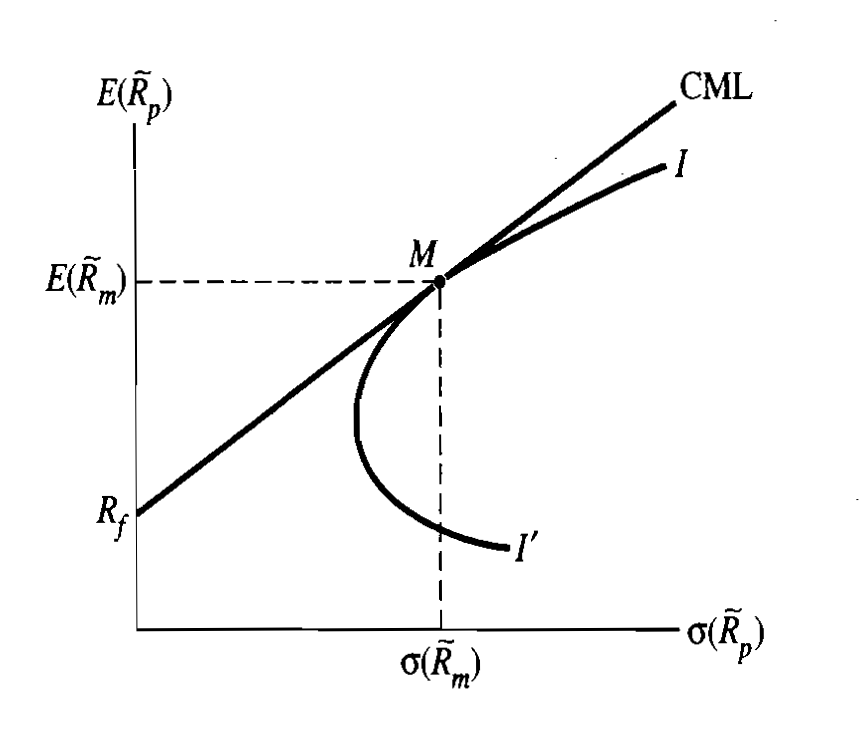
\includegraphics[width=0.5\linewidth]{screenshot015}
	\caption{The opportunity set provided by combinations of risky asset I and the market portfolio M.}
	\label{fig:screenshot015}
\end{figure}


$ IMI' $ - множество инвестиционных возможностей для комбинаций из I и М (opportunity set) 

На самом деле рыночный портфель уже включает в себя актив I, так как он включает в себя все или почти все активы рынка (высокодиверсифицированный портфель)

 Изменение ожидаемой доходности и риск портфеля P в зависимости от изменения доли вложений в риск-актив I: 
 
 \[  \dfrac{\partial E({R}_p)}{\partial a} =  E(R_i) - E(R_m) \]
 
 \[   \dfrac{\partial\sigma({R}_p)}{\partial a} = \dfrac{2a \sigma^2_{i} - (2-2a) \sigma^2_{M}  + (2-4a) \sigma_{iM} }{2\sqrt{a^2 \sigma^2_{i} + (1-a)^2 \sigma^2_{M}  + 2a(1-a) \sigma_{iM}}} \]
 
 
 $ a = 0 $, иначе существует избыточный спрос на актив I 
 
  \[   \dfrac{\partial E({R}_p) }{\partial a} \Big| _{a=0}  =  E(R_i) - E(R_m) \]
 
  \[   \dfrac{\partial\sigma({R}_p)}{\partial a} \Big| _{a=0}  = \dfrac{  \sigma_{iM} -  \sigma^2_{M}  }{\sigma_{M}  } \]
 
 
 
  Угол наклона  показывает нам  trade-off  между риском и доходностью в точке рыночного равновесия M:
  
  \[ 
  Slope =
  \dfrac{d E(R_p)}{d \sigma (R_p) } = \dfrac{E(R_i) - E(R_m) }{\dfrac{  \sigma_{iM} -  \sigma^2_{M}  }{\sigma_{M}  } } \]
  
  CAMP:
  
 \[  E(R_i) = R_f + \underbrace{\dfrac{ \sigma_{iM}}{\sigma^2_{M}}}_{\beta_i} * \underbrace{(E(R_M ) - R_f)}_{\text{премия за риск инвестирования в I }}    
  \]

 Security Market Line (SML)
 
 $ E(R_M ) - R_f $
 -  премия за риск инвестирования в I
 (премия  за риск = постоянный риск =  систематические риск = недиверсифицированный  риск) 
 
 $  \beta_i = \dfrac{ \sigma_{iM}}{\sigma^2_{M}} $  - показывает, насколько волатилен  I относительно рыночного портфеля  (насколько актив рисковый в сравнении со всеми рынком )

Доходность I никак не коррелирована  с доходностью рынка
 
 Если $ \beta_i = 0:  E(R_i ) = R_f  $
  
Если $ \beta_i = 1:  E(R_i ) = E(R_M )  $
  
  
  \begin{figure}[h!]
  	\centering
  	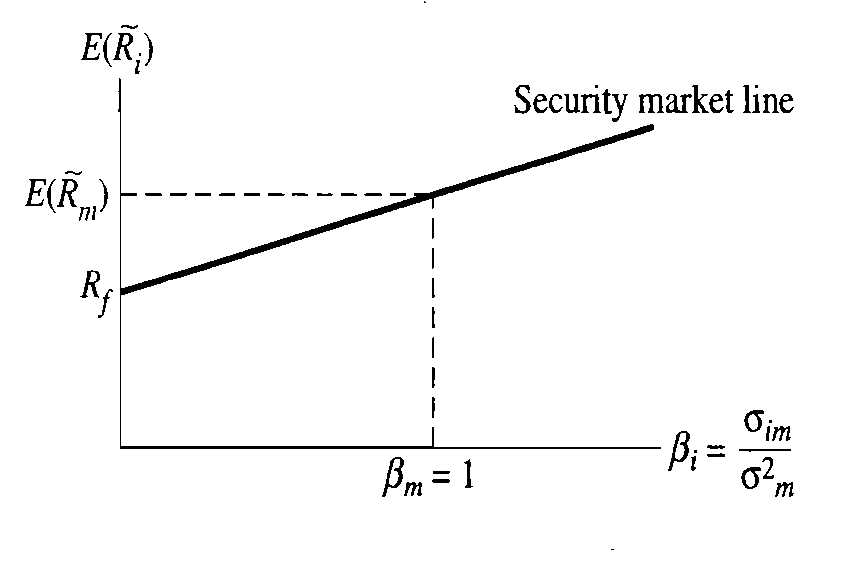
\includegraphics[width=0.6\linewidth]{screenshot016}
  	\caption{CAMP}
  	\label{fig:screenshot016}
  \end{figure}
  
  
\subsection{Влияние риска на доходность} 

Из модели CAMP следует,  что доходность $ R_i $ выражается линейным образом через доходность рыночного портфеля $R_m  $ 

\[ R_i = \alpha_i + \beta_i R_M + \varepsilon_i 
\]

где $ \varepsilon_i: E(\varepsilon_i )  = 0 $ -  влияние случайных факторов,  относящихся только к i-ому активу, а не  к рынку в целом. 

Пусть $ E[\varepsilon_i (R_M - E(R_M)) ] = 0 $ - случайные шоки и рыночная доходность не коррелируют

\[ E(R_i) = \alpha_i + \beta_i E (R_M)  
\]

\[ Cov(R_i, R_M) = E[(R_i - E(R_i))(R_M - E(R_M))]  = E[(\beta_i(R_M - E(R_M)) + \varepsilon_i) (R_M - E(R_M))] = \beta_i E[(R_M - E(R_M))^2 ] =  \beta_i \sigma^2_M \]

Откуда $ \beta_i = \dfrac{ \sigma_{iM}}{\sigma^2_{M}} $
\[ \sigma^2_{i} =  E[(R_i - E(R_i))^2 ] =  E[(\beta_i(R_M - E(R_M)) + \varepsilon_i)^2] = \beta^2_i \sigma^2_M  +  \sigma^2_\varepsilon    \]


Риск актива I складывается из риска присущего рынку в целом $ \sigma^2_M  $,   а также риска $ \sigma^2_\varepsilon     $, зависящего только от специфики конкретного актива

 Систематический рыночный риск  $ \sigma^2_M  $ -  возникает из-за внешних событий, влияющих на рынок вцелом (информационный риск,  риск негативных изменений в экономике страны вцелом).   
 Систематический риск нельзя уменьшить за счёт диверсификации, поскольку он влияет на все акции одновременно, поэтому рынок устанавливает вознаграждение за этот вид риска. 
 
 Несистематический риск $ \sigma^2_\varepsilon     $ -  диктуется событиями, связанными с самой компанией 
 (отраслевой риск -  риск, связанный с негативным влиянием на компанию отраслевых факторов,  деловой риск (business risk) - риск, связанный с неэффективностью производства и ошибками в управлении компанией)  
 
 Рассмотрим портфель,  состоящий из n активов,  доходность которого равна $ R_p $ 
 
 \[ R_p =   \sum_{i=1}^{N} x_i R_i  = \sum_{i=1}^{N} x_i (\alpha_i + \beta_i R_M + \varepsilon_i )  \]

где $ \sum_{i=1}^{N} x_i = 1 $

\[ E(R_p) =   \sum_{i=1}^{N} x_i E(R_i)  = \sum_{i=1}^{N} x_i (\alpha_i + \beta_i E(R_M) )  \]
 
  Будем считать,  что портфель достаточно диверсифицирован,   поэтому ковариация идиосинкратических активов равна 0
  
   \[ \sigma^2_{P} =  E[(R_p - E(R_p))^2 ] =  E[( \sum_{i=1}^{N} x_i \beta_i(R_M - E(R_M)) +   \sum_{i=1}^{N} x_i \varepsilon_i)^2] =   (\sum_{i=1}^{N} x_i \beta_i)^2  \sigma^2_M  +   \sum_{i=1}^{N} x_i^2 E( \varepsilon_i^2 )    \] 
  
  
  
 Рассмотрим портфели, в которых все активы имеют одинаковое веса $  x_i = \dfrac{1}{n}  $ -  случай очень хорошо диверсифицированного портфеля 
 
 
  \[ \sigma^2_{P} =    (\sum_{i=1}^{N} \dfrac{1}{n}  \beta_i)^2  \sigma^2_M  +  \dfrac{1}{n}  \sum_{i=1}^{N} \dfrac{1}{n}  E( \varepsilon_i^2 ) \xrightarrow{d}  \bar{\beta}^2 \sigma^2_M + 0 * \bar{\sigma}^2_\varepsilon  =   \bar{\beta}^2 \sigma^2_M \] 
 
 
Если портфель хорошо диверсифицирован, то весь  риск портфеля   сводится к рыночному.  
Причем, чем выше $ \beta $ (чем более волатилен портфель),  тем выше будут риски  вцелом

 Величина премии за  систематически риск: $ \beta_i [E(R_M ) - R_f]  $ - пропорциональна $ \beta $, т.е.  пропорциональна степени корреляции i-ого актива с рыночным портфелем 
 
 Если актив не коррелирует с рынком,  то его $ \beta_i = 0 \Rightarrow $ премия за риск также равна нулю 
 
  \subsection{Эмпирическая проверка модели CAMP} 
  
  Цель: адекватно описать динамику цен 
  
 \subsubsection*{  Критика модели: 
   }
   
   \begin{enumerate}
   	\item     Проблема рационального инвестора 
   	\item  Проблем асимметрии информации 
   	\item  Проблема существования банковского актива с положительной доходностью 
   	\item  Проблема существования рыночного трения ( фондовый индекс $ \neq $ рыночный портфель), при этом 
   	индивид также может инвестировать в недвижимость,  человеческий капитал и так далее 
   	\item Существование  налоговых  вычетов и транзакционных  издержек 
   	\item Проблема  "постоянного" коэффициента $ \beta $  (может быть нестабильна, от трёх лет)  
   	\item Проблема эндогенности (пропущенных переменных)


   \end{enumerate}

\end{document}